\documentclass[tikz]{standalone}
\usepackage{tikz}
% \usepackage{geometry}

% \geometry{
%   paperwidth=10in,
%   paperheight=4.5in,
%   margin=0.0in
% }

\begin{document}

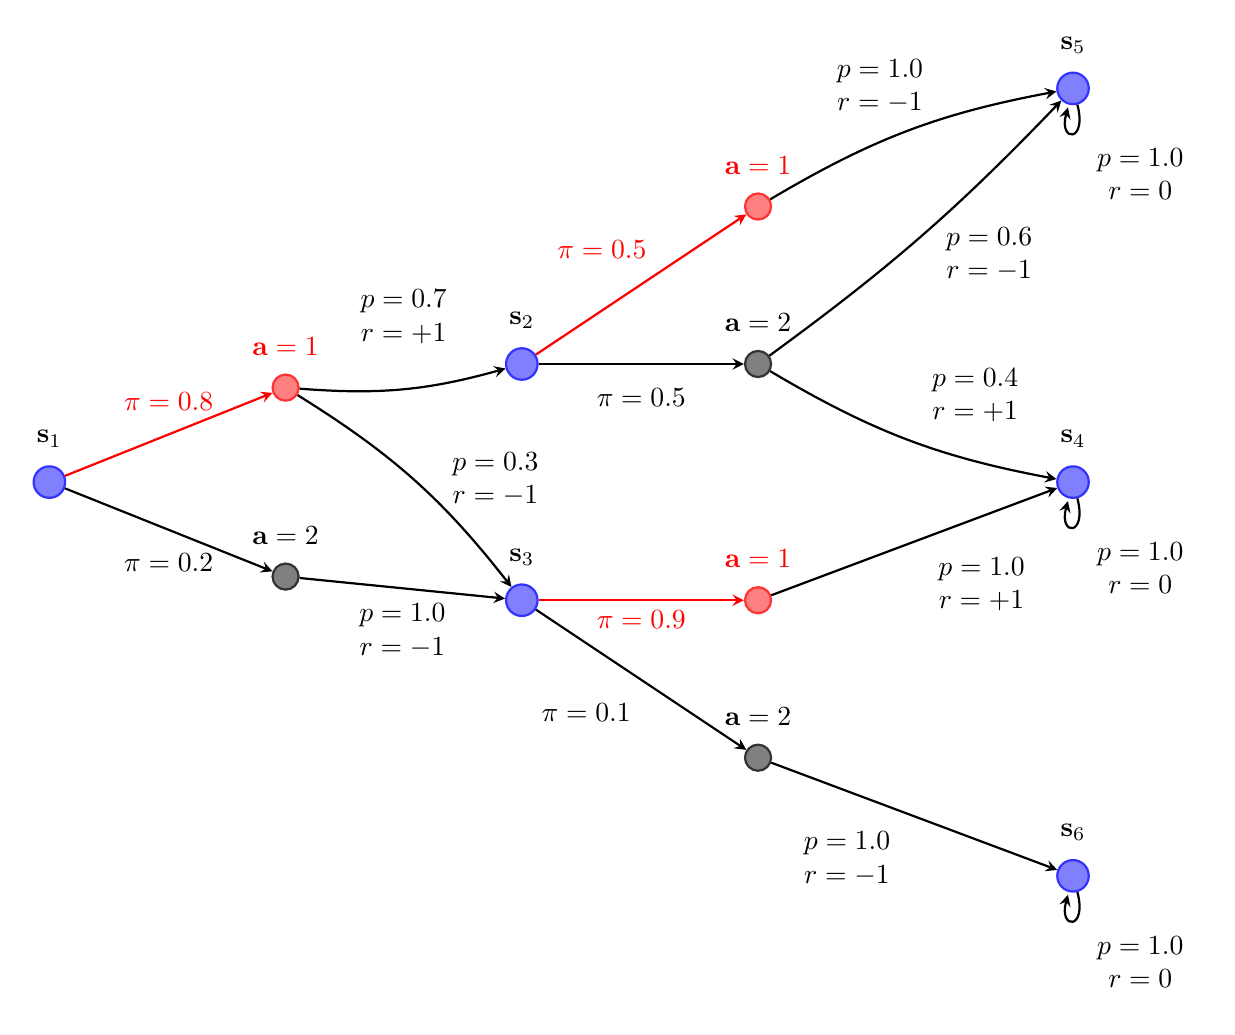
\begin{tikzpicture}[->, >=stealth, thick]

    %styles
    \tikzstyle{state}=[circle, draw=blue!80, fill=blue!50, thick, minimum size=4mm]
    \tikzstyle{action1}=[circle, draw=red!80, fill=red!50, thick, minimum size=1mm]
    \tikzstyle{action2}=[circle, draw=black!80, fill=black!50, thick, minimum size=1mm]

    % nodes
    \node[state] (s1) at (0,0) [label={[yshift=1mm]above: $ \mathbf{s}_1 $}] {};
    \node[action1] (a11) at (3, 1.2)  [label={[yshift=1mm]above: $\color{red} \mathbf{a} = 1$}] {};
    \node[action2] (a12) at (3, -1.2) [label={[yshift=1mm]above: $ \mathbf{a} = 2 $}] {};
    \node[state] (s2) at (6,1.5) [label={[yshift=1mm]above: $ \mathbf{s}_2 $}] {};
    \node[state] (s3) at (6,-1.5) [label={[yshift=1mm]above: $ \mathbf{s}_3 $}] {};
    \node[state] (s4) at (13,0) [label={[yshift=1mm]above: $ \mathbf{s}_4 $}] {};
    \node[state] (s5) at (13,5) [label={[yshift=1mm]above: $ \mathbf{s}_5 $}] {};
    \node[state] (s6) at (13,-5) [label={[yshift=1mm]above: $ \mathbf{s}_6 $}] {};
    \node[action1] (a21) at (9, 3.5)  [label={[yshift=1mm]above: $\color{red} \mathbf{a} = 1$}] {};
    \node[action2] (a22) at (9, 1.5) [label={[yshift=1mm]above: $ \mathbf{a} = 2 $}] {};
    \node[action1] (a31) at (9, -1.5)  [label={[yshift=1mm]above: $\color{red} \mathbf{a} = 1$}] {};
    \node[action2] (a32) at (9, -3.5) [label={[yshift=1mm]above: $ \mathbf{a} = 2 $}] {};
    % arrows
    \draw[red] (s1) -- node[above=5, midway] {\( \pi = 0.8 \)} (a11) ;
    \draw[black] (s1) -- node[below=5, midway] {\( \pi = 0.2 \)} (a12) ;
    \draw[black, thick, bend right=10] (a11) to node[above=10, midway] {\(\begin{array}{c} p = 0.7 \\ r = +1 \end{array}\)} (s2) ;
    \draw[black, thick, bend left=10] (a11) to node[right=5, midway] {\(\begin{array}{c} p = 0.3 \\ r = -1 \end{array}\)} (s3) ;
    \draw[black, thick, bend left=10] (a12) -- node[midway, below] {\(\begin{array}{c} p = 1.0 \\ r = -1 \end{array}\)} (s3);
    \draw[red] (s2) -- node[midway, above left, xshift=2mm, yshift=2mm] {\( \pi = 0.5 \)} (a21);
    \draw[black] (s2) -- node[below=5, midway] {\( \pi = 0.5 \)} (a22) ;
    \draw[red] (s3) -- node[midway, below] {\( \pi = 0.9 \)} (a31);
    \draw[black] (s3) -- node[below=5, below left] {\( \pi = 0.1 \)} (a32) ;
    \draw[black, thick, bend right=10] (a22) to node[above right, midway] {\(\begin{array}{c} p = 0.4 \\ r = +1 \end{array}\)} (s4) ;
    \draw[black, thick, bend right=5] (a22) to node[below right, midway, yshift=3mm] {\(\begin{array}{c} p = 0.6 \\ r = -1 \end{array}\)} (s5) ;
    \draw[black, thick, bend left=10] (a21) to node[above left, midway, xshift=5mm] {\(\begin{array}{c} p = 1.0 \\ r = -1 \end{array}\)} (s5) ;

    \draw[black, thick] (a31) -- node[below right, midway] {\(\begin{array}{c} p = 1.0 \\ r = +1 \end{array}\)} (s4) ;
    \draw[black, thick] (a32) -- node[below left, midway] {\(\begin{array}{c} p = 1.0 \\ r = -1 \end{array}\)} (s6) ;
    \draw[black, thick] (s5) edge [loop below] node[below right] {\(\begin{array}{c} p = 1.0 \\ r = 0 \end{array}\)} (s5);
    \draw[black, thick] (s4) edge [loop below] node[below right] {\(\begin{array}{c} p = 1.0 \\ r = 0 \end{array}\)} (s4);
    \draw[black, thick] (s6) edge [loop below] node[below right] {\(\begin{array}{c} p = 1.0 \\ r = 0 \end{array}\)} (s6);
\end{tikzpicture}

\end{document}
